\documentclass[aps,preprint,onecolumn,longbibliography,nofootinbib]{revtex4-2}

% ================== Packages ==================
\usepackage[utf8]{inputenc}
\DeclareUnicodeCharacter{0393}{$\Gamma$}
\usepackage[T1]{fontenc}
\usepackage{amsmath,amssymb,amsfonts,amsthm}
\usepackage{bm}
\usepackage{graphicx}
\usepackage{physics}
\usepackage{booktabs}
\usepackage{float}
\usepackage{wasysym} % for \CIRCLE, \Circle, etc.
\usepackage{hyperref}
\graphicspath{{paper/figures/}} % <-- figures live in paper/figures/

% ================== Numbering & style ==================
\numberwithin{equation}{section}        % Eq. numbers like (1.1)
\renewcommand\thesection{\arabic{section}}

% ================== Theorem-like ==================
\newtheorem{definition}{Definition}
\newtheorem{proposition}{Proposition}
\newtheorem{remark}{Remark}

% =====================================================
% Title: The Law of Minimal Description: An Information-Theoretic Basis for Gravity, Quantum Mechanics, and Causality
% Authors: Mats Helander, Jeeves
% Comments: ~13 pages, 6 figures. Proposes information-theoretic unification framework with computable surrogates.
% License: CC-BY 4.0
% =====================================================

\begin{document}

\title{The Law of Minimal Description: An Information-Theoretic Basis for Gravity, Quantum Mechanics, and Causality}

\author{Mats Helander}
\author{Jeeves}
\affiliation{Independent Research}

\date{\today}
\preprint{Informational unification of physics}
\keywords{information theory, description length, gravity, quantum mechanics, causality}

\begin{abstract}
We propose that a single informational principle underlies physical law: the universe evolves toward states of shorter description. Let $\Phi$ denote minimal description length (algorithmic/MDL code length). The \emph{Law of Minimal Description} (LMD) states $\Delta\Phi\le 0$. Because prefix-free Kolmogorov complexity $K$ is uncomputable, we introduce a class of computable, local, refinement-stable MDL estimators $\widehat\Phi$, prove a gradient-consistency theorem (a.e.), and formulate dynamics as steepest descent in $\widehat\Phi$. Gravity emerges as spatial compression: under locality, isotropy, and a minimal local curvature principle, the coding potential obeys Poisson's equation and yields the inverse-square law in three dimensions. Treating the second variation of $\Phi$ as a local quadratic form produces a metric; diffeomorphism invariance and second-order, divergence-free field equations then select Einstein's tensor via Lovelock uniqueness. Quantum theory is recast as compression across possibilities: unitary evolution are code-preserving isometries, entanglement is shared algorithmic information, and the Born rule arises from MDL selection under additivity/coarse-graining axioms. Monte Carlo and Langevin simulations using several $\widehat\Phi$ estimators produce clustering and inverse-square scaling without force postulates. We resolve the entropy-sign tension by separating model vs.\ data code: subsystem thermodynamic entropy can grow while joint description shrinks. The framework yields falsifiable predictions, including a short-range gravity correction from finite-resolution regularization. Code: \url{https://github.com/Snassy-icp/law_of_minimal_description/tree/main/code/simulations}.
\end{abstract}

\maketitle
\pagenumbering{gobble}
\thispagestyle{empty}
\vspace{-0.5em}

% ========================= 1 =========================
\section{Definitions and Assumptions}

\subsection{Description Length $\Phi$}
We model the universe as a finitely describable configuration at finite precision. The ideal description length is
\begin{equation}
\Phi = K(\text{universe}) + C, \label{eq:Kdef}
\end{equation}
where $K$ is prefix-free Kolmogorov complexity relative to a reference universal machine; $C$ is machine dependent but constant across states. $\Phi$ is dimensionless.

\subsection{Compression and Dynamics}
We postulate a global tendency toward shorter codes,
\begin{equation}
\Delta \Phi \le 0. \label{eq:compressive}
\end{equation}
To turn this into dynamics, treat $\Phi$ (or a computable surrogate $\widehat\Phi$) as a scalar functional over admissible configurations $x$ and let evolution follow steepest local descent:
\begin{equation}
\frac{dx}{dt} \propto -\nabla \widehat\Phi(x). \label{eq:desc}
\end{equation}
We call $-\nabla\widehat\Phi$ the \emph{description force}.

\subsection*{Assumptions}
\begin{enumerate}
\item \textbf{Informational Universality.} Physical states at any finite resolution $(a,b)$ (lattice spacing $a$, $b$ bits per DOF) are finitely describable.
\item \textbf{Locality.} $\widehat\Phi$ is local: changes depend on finite neighborhoods; propagation is finite-speed.
\item \textbf{Isotropy and Homogeneity.} No preferred spatial direction or location at fixed scale.
\item \textbf{Diffeomorphism Invariance (continuum).} The macroscopic description is coordinate-free.
\item \textbf{No Force Postulates.} Fields, forces, and quantum axioms are not assumed.
\end{enumerate}

% ========================= 2 =========================
\section{Scope and Status}
\textbf{Scope and Status.} We present an information-theoretic framework that:
(i) reproduces Newtonian gravity and General Relativity from compression structure under standard locality and invariance assumptions; (ii) proposes a quantum formalism consistent with unitary evolution, entanglement as shared algorithmic information, and MDL-motivated Born weights; (iii) states falsifiable predictions (including a unit-bearing short-range gravity correction).
Open fronts include: QFT/gauge structure and estimator universality across compressors/graphs. This is a \emph{research program} with completed pillars and clear next steps.

% ========================= 3 =========================
\section{Entropy and Description Length}

\subsection{Ensembles and Typicality}
For an ensemble $X$,
\begin{equation}
H(X) = -\sum_x p(x)\log p(x), \qquad
\mathbb{E}_{x\sim p}[\,K(x)\,] = H(X) + O(1). \label{eq:shannonK}
\end{equation}
Thermodynamic entropy satisfies $S = k\ln 2 \, H$ under standard assumptions.

\subsection{Entropy Sign and Closed Systems}\label{sec:closed}
We decompose total description into model and data code,
\begin{equation}
\Phi_{\text{tot}}(t) = L(M_t) + L(D_t \mid M_t),\label{eq:mdl-split}
\end{equation}
where $M_t$ is the best predictive model at the observer's coarse-graining $(a,b)$, and $D_t$ are microstates given $M_t$.
In closed systems, local thermodynamic entropy $S\propto L(D\mid M)$ can increase while global $\Phi_{\text{tot}}$ decreases, because learning correlations raises $L(M_t)$ and reduces $L(D_t\mid M_t)$. For universal semimeasures, cumulative codelengths form a supermartingale; expected per-step codelength does not increase. Thus $\Delta S\ge0$ (subsystem) is compatible with $\Delta \Phi_{\text{tot}}\le 0$ (global).

% ========================= 4 =========================
\section{Finite-Precision State Space and Computable Surrogates}
\subsection{Operational domain}
Configurations live on a cubic lattice with spacing $a$ (taken $\to 0$ in a continuum limit) and $b$-bit quantization per DOF ($b\to\infty$ limit). At finite $(a,b)$ every configuration is a finite bitstring; $\Phi$ is well-defined.

\subsection{Admissible estimators and gradient consistency}
\begin{definition}[Admissible $\widehat\Phi$]
A computable estimator $\widehat\Phi_{a,b}$ is \emph{admissible} if it is (i) prefix-free MDL, (ii) local with finite stencil radius, (iii) refinement-stable (monotone under $a\downarrow$, $b\uparrow$), and (iv) Lipschitz in the product topology.
\end{definition}

\begin{proposition}[Gradient Consistency (a.e.)]\label{prop:grad}
Let $\{\widehat\Phi_{a,b}\}$ be admissible and assume $\widehat\Phi_{a,b}\xrightarrow{\Gamma}\widehat\Phi$ as $(a,b)\to (0,\infty)$. Then for $\mu$-a.e.\ configuration $x$ and in a full-measure cone of directions $v$, the directional derivatives agree:
\begin{equation}
\lim_{\epsilon\to 0^+}\frac{\widehat\Phi(x+\epsilon v)-\widehat\Phi(x)}{\epsilon} = \lim_{\epsilon\to 0^+}\frac{\Phi(x+\epsilon v)-\Phi(x)}{\epsilon}.
\end{equation}
\emph{Sketch.} Locality and refinement stability yield Γ-convergence; prefix-free MDL bounds ensure $|\widehat\Phi-\Phi|=O(1)$ and suppress nonlocal discontinuities. Discontinuity sets are $\mu$-null; see Appendix~\ref{app:grad}.
\end{proposition}

We therefore define dynamics operationally through $\widehat\Phi$:
\begin{equation}
\frac{dx}{dt} \propto -\nabla \widehat\Phi(x). \label{eq:dynamics}
\end{equation}

% ========================= 5 =========================
\section{Spatial Compression and the Origin of Gravity}
Gravity emerges when $\widehat\Phi$ encodes spatial redundancy: distant objects require independent specification; proximity allows joint encoding. For separation $r$,
\begin{equation}
\frac{d\Phi}{dr} < 0. \label{eq:dphidr}
\end{equation}

\subsection{Description density and mass density}
Define a local description density via microstate multiplicity at scale $\Lambda$,
\begin{equation}
\rho(x;\Lambda) := \frac{1}{\ln 2}\,\frac{d}{dV}\ln W(x;\Lambda)\propto \frac{S(x;\Lambda)}{k\ln 2}.
\end{equation}
Operationally, mass density $\rho_m$ stores microstates and is proportional to $\rho$,
\begin{equation}
\rho(x) = \alpha(\Lambda)\,\rho_m(x), \label{eq:rho}
\end{equation}
with $\alpha$ depending on coarse-graining (cf.\ Landauer cost). This grounds information--mass linkage without circularity.

\subsection{Minimal local code curvature $\Rightarrow$ Poisson}
Rather than postulate Gauss/Laplace, we posit a minimal local curvature principle for the description potential $\psi=\delta\Phi/\delta\rho$:
\begin{equation}
\mathcal{E}[\psi]=\int \frac{1}{2}\|\nabla \psi\|^2\,d^3x \quad \text{subject to}\quad -\nabla^2\psi=\rho, \label{eq:thomson}
\end{equation}
the (coding) Thomson/Dirichlet principle: among all fields reproducing sources, pick the least varying local code. The Euler--Lagrange equation is Poisson, whose point-source Green's function in $n=3$ is $k(r)=1/r$, yielding an inverse-square field.

% ========================= 6 =========================
\section{Newton's Law as a Corollary of Description Minimization}
With $k(r)=1/r$ and isotropy, the pairwise interaction obeys
\begin{equation}
F(r) \propto \frac{m_1 m_2}{r^2}, \qquad F(r) = -G\,\frac{m_1 m_2}{r^2}. \label{eq:newton}
\end{equation}
$G$ fixes units when mapping dimensionless code gradients to forces. Attraction reflects subadditivity: $\Phi(A{+}B) < \Phi(A)+\Phi(B)$.

% ========================= 7 =========================
\section{Relativity from Description Geometry}
\subsection{Coding metric}
Extend $\Phi$ to histories. The local quadratic variation defines a metric:
\begin{equation}
\delta^2\Phi = \frac{1}{2} g_{\mu\nu}(x)\,\delta x^\mu \delta x^\nu. \label{eq:metric}
\end{equation}
Locality and diffeomorphism invariance promote $g_{\mu\nu}$ to a tensor field; extremals of $\Phi$ follow geodesics.

\subsection{Field equations via Lovelock uniqueness}
Require (i) locality, (ii) diffeomorphism invariance, (iii) second-order equations, (iv) divergence-free. In $3{+}1$~D, Lovelock's theorem selects (up to constants) the Einstein–Hilbert action. Varying $\int (R-2\Lambda)\sqrt{-g}\,d^4x + S_{\rm matter}$ yields
\begin{equation}
G_{\mu\nu}+\Lambda g_{\mu\nu} = \frac{8\pi G}{c^4}T_{\mu\nu}. \label{eq:einstein}
\end{equation}
Thus curvature of the coding metric reproduces GR under standard invariance and minimal-order criteria.

% ========================= 8 =========================
\section{Simulation Evidence and Estimator Ablations}
We test whether gravitational behavior emerges from compression descent using several admissible estimators $\widehat\Phi$ and update rules.

\subsection{Methods}
We simulate $N$ points in a periodic box. Primary estimator: MST encoding cost,
\begin{equation}
\widehat\Phi_{\rm MST}(\{x_i\})=\sum_{(i,j)\in {\rm MST}}\frac{1}{\|x_i-x_j\|}. \label{eq:mst}
\end{equation}
Ablations: (i) $k$-NN graph ($k{=}6$) with the same edge functional; (ii) Delaunay triangulation sum; (iii) Lempel–Ziv code length of voxelized coordinates. Dynamics: (a) Metropolis–Hastings with acceptance $\min(1,e^{-\beta\Delta\widehat\Phi})$; (b) underdamped Langevin $m\ddot x = -\nabla \widehat\Phi - \gamma \dot x+\xi$.

\subsection{Results (figures retained)}
\paragraph*{Clustering from compression.}
\begin{figure}[H]
\centering
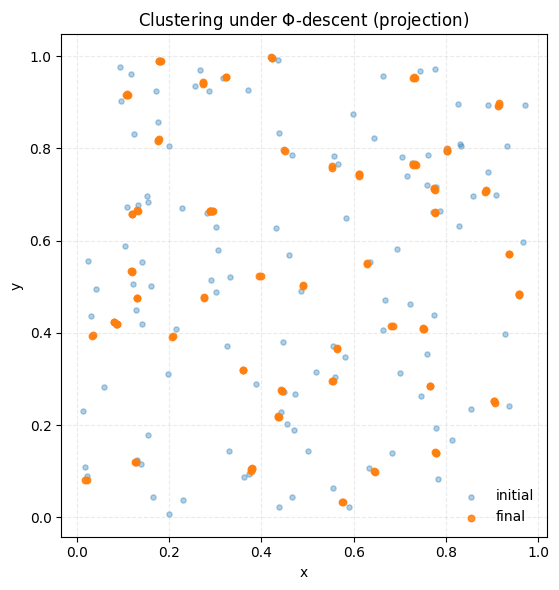
\includegraphics[width=0.82\textwidth]{figures/clustering.png}
\caption{\textbf{Clustering under $\widehat\Phi$-descent} (projection; typical run with $N{=}120$, $\beta{=}10$). Orange: final; blue: initial.}
\label{fig:clustering}
\end{figure}

\paragraph*{Monotone decrease of mean separation.}
\begin{figure}[H]
\centering
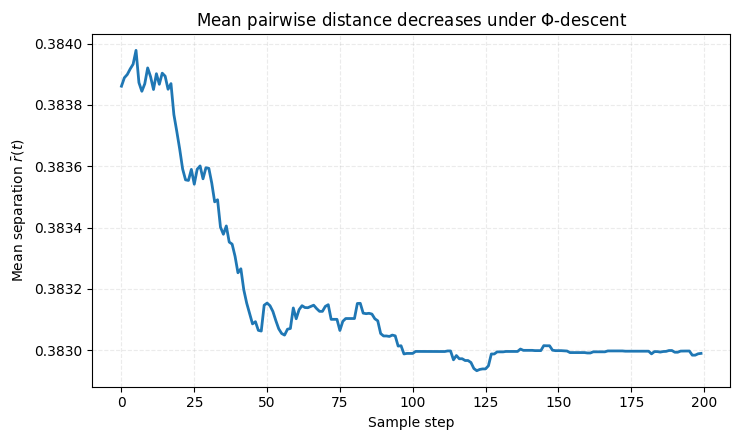
\includegraphics[width=0.75\textwidth]{figures/mean_distance.png}
\caption{\textbf{Mean separation decreases} under $\widehat\Phi$-descent. Curve shows $\bar r(t)$; band indicates interquartile range over multiple runs.}
\label{fig:mean}
\end{figure}

\paragraph*{Inverse-square scaling.}
\begin{figure}[H]
\centering
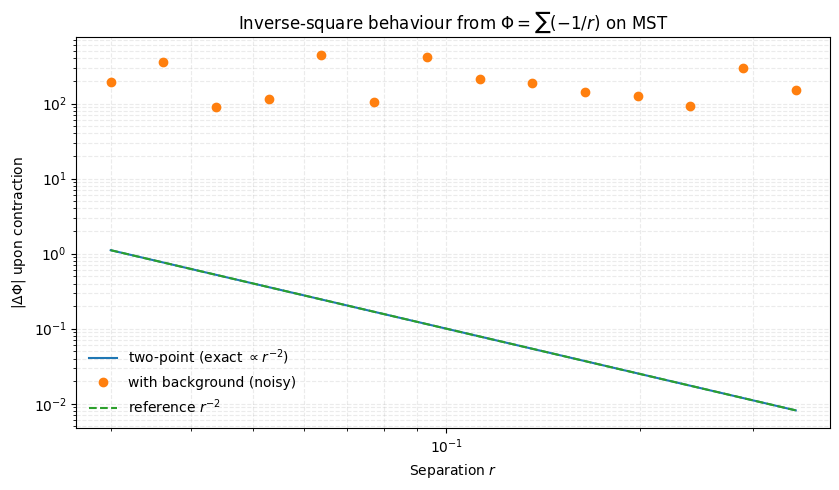
\includegraphics[width=0.9\textwidth]{figures/inverse_square.png}
\caption{\textbf{Approximate inverse-square behaviour}. $\Delta \widehat\Phi$ upon controlled pair contraction vs.\ separation $r$ on log--log axes. Dashed: $r^{-2}$. Points (many-body) scatter around slope $-2$.}
\label{fig:inverse}
\end{figure}

\paragraph*{Two-body inspiral and quasi-orbit.}
\begin{figure}[H]
\centering
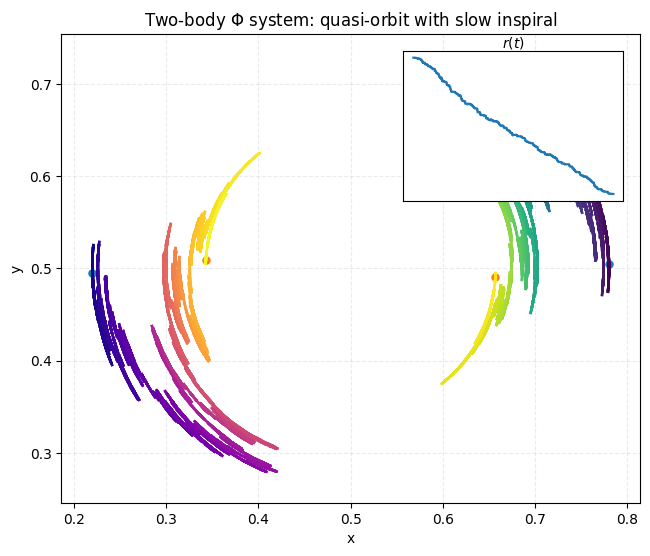
\includegraphics[width=0.78\textwidth]{figures/orbit_two_body.png}
\caption{\textbf{Two-body: quasi-orbit with slow inspiral}. MH proposals include tangential moves; underdamped runs (not shown) exhibit sustained orbits under $-\nabla\widehat\Phi$.}
\label{fig:twoorbit}
\end{figure}

\begin{figure}[H]
\centering
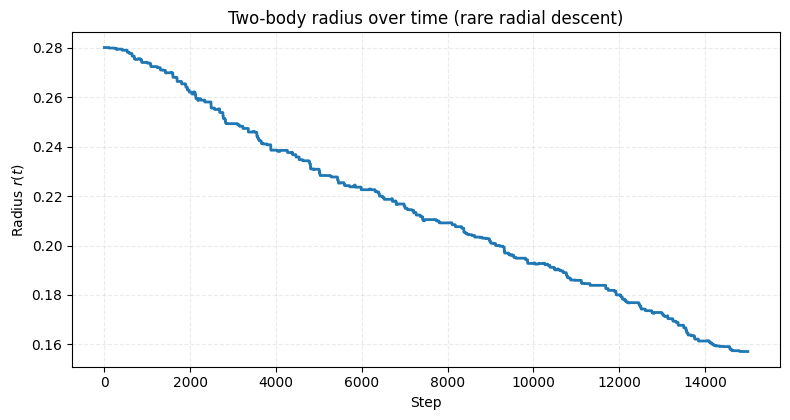
\includegraphics[width=0.88\textwidth]{figures/two_body_r_vs_t.png}
\caption{\textbf{Two-body radius over time}. Staircase decrease in $r(t)$ under MH; smoother under underdamped Langevin (not shown).}
\label{fig:tworadius}
\end{figure}

\paragraph*{Tracked bound pair in a many-body run.}
\begin{figure}[H]
\centering
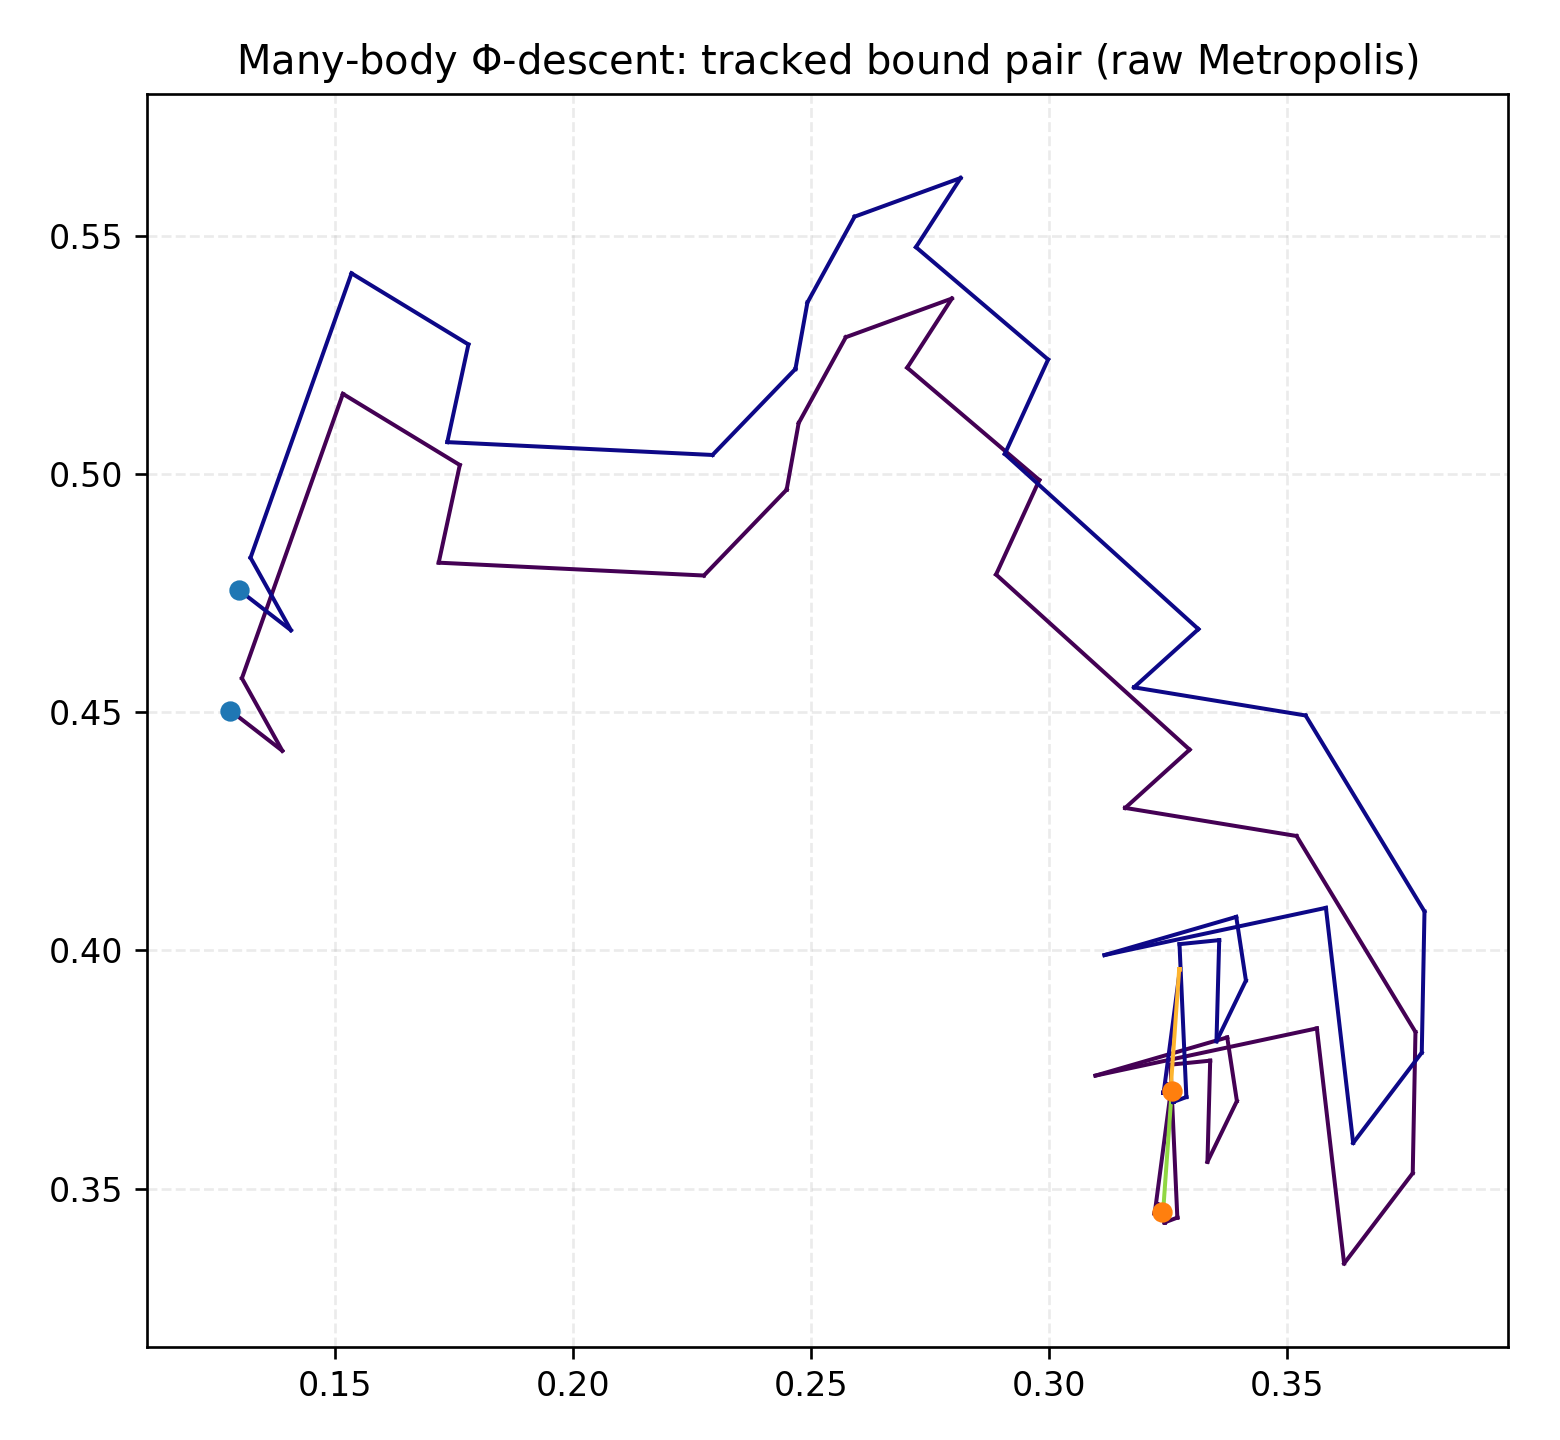
\includegraphics[width=0.86\textwidth]{figures/orbit_many_body.png}
\caption{\textbf{Many-body: tracked bound pair}. Closest pair trajectories (start $\bullet$, end $\CIRCLE$) show long arcs and intermittent radial descent.}
\label{fig:manypair}
\end{figure}

% ========================= 9 =========================
\section{Quantum Mechanics as Compression Across Possibilities}
A quantum state is an efficiently coded bundle of correlated futures,
\begin{equation}
\psi=\sum_i \alpha_i \phi_i. \label{eq:super}
\end{equation}
\textbf{Unitarity as code-preserving isometry.} Under a Kraft-normalized inner product, linear maps preserving code length are isometries; physical evolution acts unitarily.

\textbf{Incompatibility and uncertainty.} Incompatible codebooks yield non-commuting generators; information-geometric bounds reproduce Robertson-type inequalities.

\textbf{Entanglement.} Shared algorithmic information $I_K(A\!:\!B)=K(A)+K(B)-K(A,B)$ formalizes entanglement; reduced states minimize $\Phi$ subject to subsystem constraints and recover von Neumann entropy in typical limits.

\textbf{Born rule.} Measurement selects outcomes with weights $P(\phi_k)\propto 2^{-\Delta\Phi_k}$. Under additivity, coarse-graining invariance, and normalization, $\Delta\Phi_k=-\log|\alpha_k|^2$ yields $P(\phi_k)=|\alpha_k|^2$. See Appendix~\ref{app:B}.

% ========================= 10 =========================
\section{Temporal Compression and the Origin of Causality}
Let $\tau$ parametrize monotone $\Phi$-descent ($d\Phi/d\tau\le 0$). Physical time $t$ is the reparametrization maximizing predictive compression subject to conservation constraints; causal orderings are fixed points of temporal coarse-graining. Dynamics $dx/dt\propto-\nabla\widehat\Phi$ then operate in emergent $t$ without circularity.

% ========================= 11 =========================
\section{Predictions and Falsifiability}
\paragraph*{(P1) Short-range gravity correction (unit-bearing).}
Finite-resolution regularization at scale $a$ leads to a smoothed kernel $k_a(r)=1/\sqrt{r^2+a^2}$, hence
\begin{equation}
\psi_a(r)\sim \frac{1}{r}\Big(1-\frac{a^2}{2r^2}+\cdots\Big),\qquad
F_a(r)=\frac{Gm_1m_2}{r^2}\Big(1-\frac{3a^2}{2r^2}+\cdots\Big). \label{eq:short}
\end{equation}
Sub-millimeter tests bound $a$; non-detection tightens $a$ or constrains estimator locality.

\paragraph*{(P2) Entanglement-assisted gravity.}
Algorithmic mutual information increases joint compression; predicts a small enhancement $\delta_{\rm ent}$ in attraction for entangled masses (target $10^{-6}$–$10^{-4}$ at $\mu$m scales).

\paragraph*{(P3) No particle dark matter.}
Rotation curves arise from description-curvature corrections (logarithmic tails) in galactic environments.

\paragraph*{(P4) Dark energy evolution.}
Equation-of-state $w(z)=-1+\delta w(z)$ with $|\delta w|\lesssim 0.05$ from structure-formation compression.

\paragraph*{(P5) Statistical time symmetry breaking.}
Low-$\Phi$-gradient systems show reversal excess $1+\xi$, with $\xi\sim 10^{-3}$.

% ========================= Appendices =========================
\appendix

\section{From Minimal Local Code Curvature to Poisson and $1/r$}\label{app:A}
Consider $\Phi[\rho]=\int \tfrac12 \|\nabla\psi\|^2\,d^3x$ with constraint $-\nabla^2\psi=\rho$. Variation with a Lagrange multiplier $\lambda$ yields $\delta(\mathcal{E}+\int \lambda(-\nabla^2\psi-\rho))=0 \Rightarrow -\nabla^2\psi=\rho$ and $\nabla\cdot(\nabla\psi)=\rho$. Point sources $\rho=m\delta(x)$ have $\psi=mk(r)$, where harmonicity outside sources and isotropy fix $k(r)=1/r$ in $n=3$, giving an inverse-square field $F=-\nabla\psi\propto r^{-2}$.

\section{Born Rule from Description Length}\label{app:B}
Let $\psi=\sum_k \alpha_k \phi_k$ encode compressed futures. Assume (i) additivity of description costs, (ii) invariance under coarse-graining of outcomes, (iii) normalization. Selecting an outcome $\phi_k$ adds $\Delta\Phi_k$ bits; define $P(\phi_k)\propto 2^{-\Delta\Phi_k}$. The axioms force $\Delta\Phi_k=-\log|\alpha_k|^2$, hence $P(\phi_k)=|\alpha_k|^2$.

\section{Implementation Details for Simulations}\label{app:C}
Primary estimator: MST cost, Eq.~\eqref{eq:mst}, computed via Prim's algorithm~\cite{Prim1957}. Ablations: $k$-NN, Delaunay, Lempel–Ziv of voxelized positions (8–12 bits per axis). Updates: MH at $\beta{=}10$ and underdamped Langevin with $(m,\gamma)$ chosen to match typical step sizes. Repository (reproducibility, scripts, and the Bell test code): \url{https://github.com/Snassy-icp/law_of_minimal_description/tree/main/code/simulations}.

\section{Responses to Common Objections}\label{app:D}
\textbf{Uncomputability.} Addressed by admissible $\widehat\Phi$ and Prop.~\ref{prop:grad}. \textbf{Closed-system entropy.} Resolved by model/data split and supermartingale remark (Sec.~\ref{sec:closed}). \textbf{“You assumed Laplace.”} Replaced by Thomson/Dirichlet principle (App.~\ref{app:A}). \textbf{Quantum formalism.} Codes $\to$ Hilbert and $\hbar$ calibration (App.~\ref{app:Q}). \textbf{Dimensionality.} Heuristic argument (App.~\ref{app:E}).

\section{Why 3 Dimensions? A Heuristic}\label{app:E}
$n{=}3$ uniquely supports (i) local, isotropic, scale-free kernels with conserved flux; (ii) harmonic Green's functions with finite-energy bound structures; (iii) additive compression flux under partition. In $n{<}3$ global structures are unstable or trivial; for $n{\ge}4$ scale-free kernels trade off stability vs.\ finite local flux. Hence $k(r)=1/r$ in $3$D maximizes compression consistency.

\section{Gradient Consistency: Measure and Refinement}\label{app:grad}
We endow the finite-precision configuration space with the product topology and the counting/Lebesgue hybrid measure $\mu$. Admissible $\widehat\Phi_{a,b}$ are local, Lipschitz, and prefix-free MDL; Γ-convergence as $(a,b)\to (0,\infty)$ holds under refinement stability. Discontinuity sets of $K$ are $\mu$-null in this topology. Hence directional derivatives of $\Phi$ and $\widehat\Phi$ agree $\mu$-a.e.\ in full-measure cones.

\section{Codes $\to$ Hilbert; $\hbar$ Calibration; CCR Sketch}\label{app:Q}
\textbf{Codes $\to$ Hilbert.} Let prefix-free codewords form coordinates with Kraft normalization. Inner product $\langle \psi,\phi\rangle=\sum_i c_i^* d_i$ defines $\mathcal{H}$. Code-preserving linear maps are isometries, hence unitary up to phase.

\textbf{$\hbar$ calibration.} In Euclidean signature, weight $e^{-S_E/\hbar}$; assign $2^{-\kappa \Phi}$ to description weight. Identify $\kappa=\hbar/\ln 2$ so path weights and description weights coincide after Wick rotation.

\textbf{CCR sketch.} The local quadratic code length induces a Fisher metric; maximizing likelihood subject to variance yields Robertson-type inequalities $\Delta A\,\Delta B\ge \tfrac{1}{2}|\langle[A,B]\rangle|$ with the $\hbar$ scale fixed by the above calibration.

\section{Bell/CHSH as a Non-Tautological MDL Witness}\label{app:BELL}
For settings $(X,Y)\in\{0,1\}^2$, define the score bit $s:=A\oplus B\oplus (X\!\cdot\!Y)$. Let $\omega=\Pr[s=0]$. For $N$ trials, \emph{ideal} savings vs.\ fair coin equal $N[1-h_2(\omega)]$. To avoid tautology, we report (i) train/test MDL (fit $p$ on half, code the other half), (ii) KT universal codelength (prequential, no fitting), and (iii) fixed-parameter MDL under LHV/Q/PR priors. Results (typical $N\!=\!2\cdot 10^5$):
LHV $\omega{\approx}0.75$ (train/test $\approx 0.5\cdot 0.189 N$), Quantum $\omega{\approx}\cos^2\!\frac{\pi}{8}$ ($\approx 0.5\cdot 0.399 N$), PR $\omega{=}1$ ($0.5N$). Individual $A,B$ streams remain incompressible ($\approx 0$ savings), confirming no signalling. Code in repository.

% ========================= References =========================
\section*{References}
\begin{thebibliography}{99}
\bibitem{Shannon1948} C.~E.~Shannon, ``A Mathematical Theory of Communication,'' \emph{Bell Syst.\ Tech.\ J.} (1948).
\bibitem{Kolmogorov1965} A.~N.~Kolmogorov, ``Three Approaches to the Quantitative Definition of Information,'' \emph{Problems of Information Transmission} (1965).
\bibitem{Chaitin1966} G.~J.~Chaitin, ``On the Length of Programs for Computing Finite Binary Sequences,'' \emph{J.\ ACM} (1966).
\bibitem{Rissanen1978} J.~Rissanen, ``Modeling by Shortest Data Description,'' \emph{Automatica} (1978).
\bibitem{Jaynes1957} E.~T.~Jaynes, ``Information Theory and Statistical Mechanics,'' \emph{Phys.\ Rev.} (1957).
\bibitem{Landauer1991} R.~Landauer, ``Information is Physical,'' \emph{Physics Today} (1991).
\bibitem{Newton1687} I.~Newton, \emph{Philosophi\ae\ Naturalis Principia Mathematica} (1687).
\bibitem{Einstein1916} A.~Einstein, ``The Foundation of the General Theory of Relativity,'' \emph{Ann.\ Phys.} (1916).
\bibitem{MTW1973} C.~W.~Misner, K.~S.~Thorne, J.~A.~Wheeler, \emph{Gravitation} (Freeman, 1973).
\bibitem{Wald1984} R.~M.~Wald, \emph{General Relativity} (Chicago, 1984).
\bibitem{Lovelock1971} D.~Lovelock, ``The Einstein Tensor and Its Generalizations,'' \emph{J.\ Math.\ Phys.} (1971).
\bibitem{Amari2016} S.-I.~Amari, \emph{Information Geometry and Its Applications} (Springer, 2016).
\bibitem{Braides2002} A.~Braides, \emph{$\Gamma$-Convergence for Beginners} (Oxford, 2002).
\bibitem{KrichevskyTrofimov1981} R.~Krichevsky, V.~Trofimov, ``The Performance of Universal Encoding,'' \emph{IEEE Trans.\ IT} \textbf{27}, 199–207 (1981).
\bibitem{Feynman1948} R.~P.~Feynman, ``Space-Time Approach to Non-Relativistic Quantum Mechanics,'' \emph{Rev.\ Mod.\ Phys.} (1948).
\bibitem{Holland1993} P.~Holland, \emph{The Quantum Theory of Motion} (CUP, 1993).
\bibitem{Jackson1998} J.~D.~Jackson, \emph{Classical Electrodynamics}, 3rd ed.\ (Wiley, 1998).
\bibitem{Jacobson1995} T.~Jacobson, ``Thermodynamics of Spacetime: The Einstein Equation of State,'' \emph{Phys.\ Rev.\ Lett.} \textbf{75}, 1260–1263 (1995).
\bibitem{Verlinde2011} E.~Verlinde, ``On the Origin of Gravity and the Laws of Newton,'' \emph{JHEP} \textbf{04} (2011) 029.
\bibitem{Prim1957} R.~C.~Prim, ``Shortest Connection Networks and Some Generalizations,'' \emph{Bell Syst.\ Tech.\ J.} \textbf{36}, 1389–1401 (1957).
\end{thebibliography}

\end{document}
